% Start with
\documentclass[twocolumn]{article}

% Import package for random typing
% STUDENTS: DO NOT USE THIS
\usepackage{lipsum}

% Import multicolumn package
\usepackage{multicol}

% Import geometry package to set paper sizes
\usepackage{geometry}
\geometry{a4paper, left=30mm, right=30mm, top=30mm, bottom=30mm}

% Import font package
\usepackage{fontenc}

% Import tikz
%every picture/.append style={defcoords} % will apply this to all tikzpictures
\usepackage{tikz}

% Import bibliography packages
\usepackage{natbib}
\usepackage{url}
\usepackage{hyperref}
\hypersetup{ 
colorlinks=true, 
linkcolor=blue, 
filecolor=blue, 
citecolor = black,       
urlcolor=cyan, 
} 

% Insert images
\usepackage{graphicx}
\graphicspath{{figures/}}

% Import pgfplots
\usepackage{pgfplots}

% Import text file reader
\usepackage{csvsimple}

% Import listings for Python scripts
\usepackage{listings}

% Import fancy python view packages
\usepackage{mdframed}

% Begin the document
\begin{document}

% Add title page
\begin{titlepage}

% To center everything in thi page
\centering


\includegraphics[%
    width=1.7in,
]{figures/btu_logo}%

\vspace{1cm}
{\Huge \textbf{Final Project Report }}

\vspace{1cm}
{\Huge \textbf{Sierpinski Triangle and \\ Koch Snowflake Fractals by \\ Python and Pgfplots}}

\vspace{1cm}
\LARGE Bursa Technical University \\
Department of Mechanical Engineering \\
Computer Programming Course \\


\Large
% Put some space before the names
\vspace{1cm}
\textbf{Team 0}
\begin{center}
  \begin{tabular}{ l r }
Name & Student ID \\ \hline
Levent Aydinbakar & 1234567890 \\ 
Levent Aydinbakar & 1234567890 \\ \end{tabular}
\end{center}

\vspace{1cm}
\large \textbf{Instructor:} Dr. Levent Aydinbakar \\

% Puts everything after this point
% at the end (bottom) of this page
\vfill

\begin{abstract}
\textcolor{gray}{
\lipsum[2]
}

\end{abstract}

\vspace{1cm}
\large \today

\end{titlepage}

\onecolumn
\tableofcontents
\listoffigures
\listoftables
\twocolumn

\section{Introduction}
\textcolor{gray}{
\lipsum[1-2]
}
\cite{fractalFoundation}. 



\section{Sierpinski Triangle}
\label{sec:SierpinskiTriangle}
\textcolor{gray}{
\lipsum[1-1]
}
\cite{sierpinskiWiki}.

\subsection{Sierpinski triangle by random points}
Sierpinski triangle can be obtained by randomly selected points. 
To draw it in this way one can follow the path below.

\subsubsection{Three corner points of an equilateral triangle}
An equilateral triangle is represented by its corner points first.
\begin{figure}[htb]
\centering
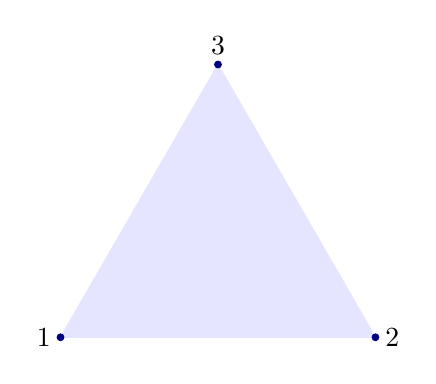
\begin{tikzpicture}
\coordinate (A) at (0,0); 
\coordinate (B) at (4,0); 
\coordinate (C) at (2,3.464);
\draw[fill, blue!10!white] (A) -- (B) -- (C) -- (A);
\draw[fill, blue!50!black] (A) circle (1.2pt) node[black,  left]{$1$};
\draw[fill, blue!50!black] (B) circle (1.2pt) node[black, right]{$2$};
\draw[fill, blue!50!black] (C) circle (1.2pt) node[black, above]{$3$};
\end{tikzpicture}
\caption{An equilateral triangle corner points}
\label{fig:threePoints}
\end{figure}

\subsubsection{Selecting a random point}
Later, a random point is choosen on the triangle.
\begin{figure}[htb]
\centering
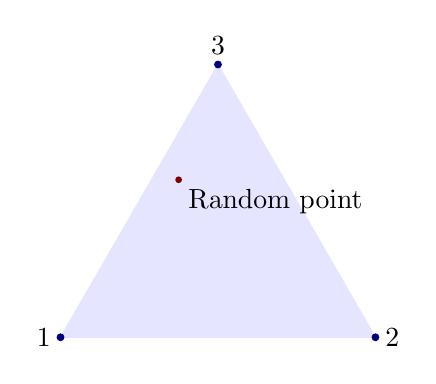
\begin{tikzpicture}
\coordinate (A) at (0,0); 
\coordinate (B) at (4,0); 
\coordinate (C) at (2,3.464);
\draw[fill, blue!10!white] (A) -- (B) -- (C) -- (A);
\draw[fill, blue!50!black] (A) circle (1.2pt) node[black,  left]{$1$};
\draw[fill, blue!50!black] (B) circle (1.2pt) node[black, right]{$2$};
\draw[fill, blue!50!black] (C) circle (1.2pt) node[black, above]{$3$};
\draw[fill, red!50!black] (1.5,2) circle (1pt)  node[black, below right]{Random point};
\end{tikzpicture}
\caption{Random point on the equilateral triangle}
\label{fig:randomPoint}
\end{figure}
\begin{figure}[hb!]
\centering
\begin{tikzpicture}
\node at (0,0.0) {\includegraphics[page=3]{midpoints.pdf}};
\node at (0,4.2) {\includegraphics[page=2]{midpoints.pdf}};
\node at (0,8.4) {\includegraphics[page=1]{midpoints.pdf}};
\end{tikzpicture}
\caption{The first midpoint is selected in the middle of the point $1$ (randomly selected) and the random point (\textit{top}).
The second midpoint is selected in the middle of the point $2$ (randomly selected) and the first midpoint (\textit{middle}).
The third midpoint is selected in the middle of the point $3$ (randomly selected) and the second midpoint (\textit{bottom})}
\label{fig:firstMidPoint}
\end{figure}

\subsubsection{Selecting a midpoint}
In the following step, a corner point is selected randomly and another point is drawn 
in the middle of this corner point and the random point (see Figure~\ref{fig:firstMidPoint}).

\begin{figure}[ht!]
\centering
\begin{tikzpicture}
\node at (0,0.0)  {\includegraphics[page=4]{iterations.pdf}};
\node at (0,4.2)  {\includegraphics[page=3]{iterations.pdf}};
\node at (0,8.4)  {\includegraphics[page=2]{iterations.pdf}};
\node at (0,12.6) {\includegraphics[page=1]{iterations.pdf}};
\end{tikzpicture}
\caption{The points after 10, 100, 1000, and 2000 iterations 
from \textit{top} to \textit{bottom}}
\label{fig:iterations}
\end{figure}
When this process is repeated for 10 times, 
100 times, 
100 times,
1000 times, and
20000 times, Figure~\ref{fig:iterations} is obtained.

\subsubsection{Method}
Figure~\ref{fig:iterations} and other fractal pictures can be obtained with some simple calculations in Python.
There are also some libraries to do it. 
However, an example script can generate the Sierpinski Triangle manually is given in Appendix~\ref{app:sierpinski}.

\textcolor{gray}{
\lipsum[2][1-7]
}

\subsection{Upside down Sierpinski triangle}
Another way of making Sierpinski triangle is explained in the following sections.

\subsubsection{Start with a triangle}
Let's use a upside down equilateral triangle first. 
Then, take its half and recombine three of the half models together to obtain the original shape
(see Figures~\ref{fig:sierpinskiWithSurfaces1},
\ref{fig:sierpinskiWithSurfaces2}, and
\ref{fig:sierpinskiWithSurfaces3}).

\begin{figure}[ht!]
\centering
\begin{tikzpicture}
\coordinate (A) at (0,0); 
\coordinate (B) at (4,0); 
\coordinate (C) at (2,-3.464);
\draw[latex-latex] (0,0.2) -- (4,0.2) node[midway, above]{$l$};
\draw[blue!50!black] (A) -- (B) -- (C) -- (A);

\coordinate (A) at (5,0); 
\coordinate (B) at (6.33,0); 
\coordinate (C) at (5.66,-1.155);
\draw[latex-latex] (5,0.2) -- (6.33,0.2) node[midway, above]{$l/2$};
\draw[blue!50!black] (A) -- (B) -- (C) -- (A);

\draw[latex-latex] (1.3,-3.8) -- (5.3,-3.8) node[midway, above]{$l$};
\node[anchor=north west] at (1.165,-4){\includegraphics{lines1.pdf}};

\end{tikzpicture}
\caption{The upside down equilateral triangle, halved model, and recombined model, from \textit{left} to \textit{right} and \textit{top} to \textit{bottom}}
\label{fig:sierpinskiWithSurfaces1}
\end{figure}


\begin{figure}[hb!]
\centering
\begin{tikzpicture}
\draw[latex-latex] (0.145,0.2) -- (4.145,0.2) node[midway, above]{$l$};
\draw[latex-latex] (5.145,0.2) -- (6.475,0.2) node[midway, above]{$l/2$};
\draw[latex-latex] (1.3,-3.8) -- (5.3,-3.8) node[midway, above]{$l$};
\node[anchor=north west] at (0,0){\includegraphics[page=1]{lines2.pdf}};
\node[anchor=north west] at (5,0){\includegraphics[page=2]{lines2.pdf}};
\node[anchor=north west] at (1.165,-4){\includegraphics[page=3]{lines2.pdf}};
\end{tikzpicture}
\caption{The equilateral triangle at the second step, halved model, and recombined model from \textit{left} to \textit{right} and \textit{top} to \textit{bottom}}
\label{fig:sierpinskiWithSurfaces2}
\end{figure}

\begin{figure}[htb!]
\centering
\begin{tikzpicture}
\node[anchor=north west] at (0,4.2){\includegraphics[page=1]{lines34567.pdf}};
\node[anchor=north west] at (0,0){\includegraphics[page=2]{lines34567.pdf}};
\node[anchor=north west] at (0,-4.2){\includegraphics[page=3]{lines34567.pdf}};
\node[anchor=north west] at (0,-8.4){\includegraphics[page=4]{lines34567.pdf}};
\node[anchor=north west] at (0,-12.6){\includegraphics[page=5]{lines34567.pdf}};
\end{tikzpicture}
\caption{The third, fourth, fifth, sixth, and seventh steps
from \textit{top} to \textit{bottom}}
\label{fig:sierpinskiWithSurfaces3}
\end{figure}

The scripts can be seen in Appendix~X.



\clearpage
\newpage
\mbox{~}
\section{Koch Snowflake}
\label{sec:KochSnowflake}

In Section~\ref{sec:SierpinskiTriangle}, we show how to make the Sierpinski Triangle.
Here we will show the Koch Snowflake \cite{KS, OP, LA}.

The Koch Snowflake can also be obtained from a equilateral triangle.

\begin{figure}[htb]
\centering
\begin{tikzpicture}
\coordinate (A) at (0,0); 
\coordinate (B) at (4,0); 
\coordinate (C) at (2,3.464);
\draw[blue!50!white] (A) -- (B) -- (C) -- (A);
\end{tikzpicture}
\caption{An equilateral triangle corner points}
\label{fig:triangleKSP}
\end{figure}

Then the lines are divided into 3 equal parts, the middle part is rotated $60^\circ$ around both of the points.

\begin{figure}[htb]
\centering
\begin{tikzpicture}
\coordinate (A) at (0,0); 
\coordinate (B) at (4,0); 
\coordinate (C) at (2,3.464);
\draw[blue!50!white] (A) -- (B) -- (C) -- (A);
\node at (2,1.15){\includegraphics{KSP1.pdf}};
\end{tikzpicture}
\caption{A first order Koch Snowflake}
\label{fig:KSP1}
\end{figure}

When we continue dividing each line and rotating the midline, we can obtain Figure~\ref{fig:KSP2}.

\textcolor{gray}{
\lipsum[2]
}

\begin{figure}[htb]
\centering
\begin{tikzpicture}
\node[anchor=north west] at (0,4.8)  {\includegraphics[page=1]{KSP2.pdf}};
\node[anchor=north west] at (0,0)    {\includegraphics[page=2]{KSP2.pdf}};
\node[anchor=north west] at (0,-4.8) {\includegraphics[page=3]{KSP2.pdf}};
\node[anchor=north west] at (0,-9.6) {\includegraphics[page=4]{KSP2.pdf}};
\end{tikzpicture}
\caption{A second, third, fourth, fifth, and sixth order Koch Snowflakes from 
from \textit{top} to \textit{bottom}}
\label{fig:KSP2}
\end{figure}

%The length of the equilateral triangle given in Figure~\ref{fig:triangleKSP} is $l$. 
%The perimeter of the triangle is defined as $3l$.
%When the rule shown in Figure~\ref{fig:KSP1} is applied, the new figure has $\frac{4}{3}l$.
%Then the perimeter of the new shape is $3\frac{4}{3}l$.
%The perimeter of the second order shape is calculated as $3\frac{4}{3}^2l$.
%When we apply the rule $n$ times, then the perimeter is defined as $3\frac{4}{3}^nl$.



\newpage
\clearpage
\section{Fractals with Pgfplots}
There is a library of Pgfplots to draw fractals.
For example see Appendix~\ref{app:kspgf} for the script
to draw Figure~\ref{fig:KSPgf}


\begin{figure}[ht!]
\centering
\begin{tikzpicture}
\node at (5,0)  {\includegraphics[scale=1]{KSPPgf.pdf}};
\end{tikzpicture}
\caption{
A Koch Snowflake drawn using Pgfplots}
\label{fig:KSPgf}
\end{figure}

\textcolor{gray}{
\lipsum[2][3-5]
}

\begin{figure}[ht!]
\centering
\begin{tikzpicture}
\node at (0,0)  {\includegraphics[scale=2.5]{hexaPgf.pdf}};
\end{tikzpicture}
\caption{
A hexagon fractal drawn using Pgfplots}
\label{fig:hexa}
\end{figure}

\textcolor{gray}{
\lipsum[2][1-2]
}

\begin{figure}[ht!]
\centering
\begin{tikzpicture}
\node at (0,0)  {\includegraphics[scale=2.5]{treePgf.pdf}};
\end{tikzpicture}
\caption{
A tree drawn using Pgfplots}
\label{fig:tree}
\end{figure}

\textcolor{gray}{
\lipsum[2-3]
}


\begin{table*}[ht!]
\caption{Contribution of each team member}
\label{tb:contribute}
%\begin{tabular}{|wl{0.79\textwidth} |wl{0.79\textwidth} | wc{0.06\textwidth}| }
\begin{tabular}{l l l }
Part & Member(s) & Contribution rate \\
Python scripts & Levent Aydinbakar & $70~\%$ \\
Python scripts & Other Student & $30~\%$ \\
Shell scripts & Levent Aydinbakar & $100~\%$ \\
Gnuplot scripts & Levent Aydinbakar & $100~\%$ \\
Pgfplots graphs & Levent Aydinbakar & $100~\%$ \\
Tikz sketches & Levent Aydinbakar & $100~\%$ \\
\LaTeX{} scripts & Levent Aydinbakar & $100~\%$ \\
Research of the subject & Levent Aydinbakar & $100~\%$ \\
\end{tabular}
\end{table*}

\section{Contibutions}
\label{sec:contributions}

Contributions of each team member in this report is given in Table~\ref{tb:contribute}.


\section{Conclusions}
\textcolor{gray}{
\lipsum[1-1]
}





\newpage
\newpage
\onecolumn
\bibliographystyle{unsrt}
\bibliography{ref.bib}

\appendix
\newpage
\section{Sierpinski Triangle by Python}
\label{app:sierpinski}
\begin{mdframed}
\small
\begin{verbatim}
#!/usr/bin/env python3
# Import necessary modules
import numpy
import math
import random
import argparse

# Argument parser to read info from commandline
parser = argparse.ArgumentParser()
parser.add_argument("-i","--iterations", \
                    default=100, type=int, \
                    help="Number of iterations (=100).")
args = parser.parse_args()

# Define length
l=4

# A function to rotate a point around another point
def rotate(point, origin, degrees):
  radians = numpy.deg2rad(degrees)
  x,y = point
  offset_x, offset_y = origin
  adjusted_x = (x - offset_x)
  adjusted_y = (y - offset_y)
  cos_rad = numpy.cos(radians)
  sin_rad = numpy.sin(radians)
  qx = offset_x + cos_rad * adjusted_x - sin_rad * adjusted_y
  qy = offset_y + sin_rad * adjusted_x + cos_rad * adjusted_y
  return qx, qy

# Make the triangle
p1=numpy.array([0,0])
p2=numpy.array([l,0])
p3=rotate(p2, p1, 60)

# Put a random point
random_point=numpy.array([1.5,2])

# Make a tuple to select p1, p2 or p3 randomly
r=numpy.stack((p1,p2,p3))

# Add the first point
p=numpy.vstack((p1,p2,p3,(p1+random_point)/2))

# Add the other points
for i in range(args.iterations):
  pp=random.choice(r)
  pnew=(pp+p[-1])/2
  p=numpy.vstack((p, pnew))

# Save the points to a file
# Add header x,y for Tikz
with open("sierpinski_points.txt","w") as f:
  f.write("x,y\n")
  numpy.savetxt(f, p, fmt="%1.5f", delimiter=",")
\end{verbatim}
\end{mdframed}

\newpage
\section{Koch Snowflake by Pgfplots}
\label{app:kspgf}

\begin{mdframed}
\small
\begin{verbatim}

\documentclass[tikz,margin=2mm]{standalone}
\usepackage{tikz}

\usetikzlibrary{lindenmayersystems}

\begin{document}%
\def\hexagwidth{4cm}%
\pgfdeclarelindenmayersystem{Sierpinski hexagon}{
  \symbol{X}{\pgflsystemdrawforward}
    \symbol{Y}{\pgflsystemmoveforward\pgflsystemmoveforward\pgflsystemmoveforward}
    \rule{X -> X+X+X+X+X+X+Y}
    \rule{Y -> YYY}
}%
\foreach \level in {4,...,4}{%
\tikzset{
    l-system={step=\hexagwidth/3^\level, order=\level, angle=60}
}%
\begin{tikzpicture}
%  \fill[blue!50!black] (0,0) l-system 
\shadedraw [top color=white, bottom color=blue!50!black, draw=blue!50!black]
l-system
  [l-system={Sierpinski hexagon, axiom=X}] ;
\end{tikzpicture}
}%
\end{document}

\end{verbatim}
\end{mdframed}




% The document finishes here
\end{document}

